\chapter{Introduction}

%Provide a short summary of the whole PhD thesis:
% -Introduction to QC & CQED
% -Building Blocks of Superconducting Quantum Processors
% -Realization of a 2-Transmon QP
% -Tune-Up & Characterization of the Universal 2-Qubit Gate
% -Grover's Algorithm: Introduction & Background
% -Implementation on the 2-Qubit Processor
% -Design of a Scalable QC Architecture

\section{Quantum Computing \& Circuit Quantum Electrodynamics}

\begin{figure}
	\centering
		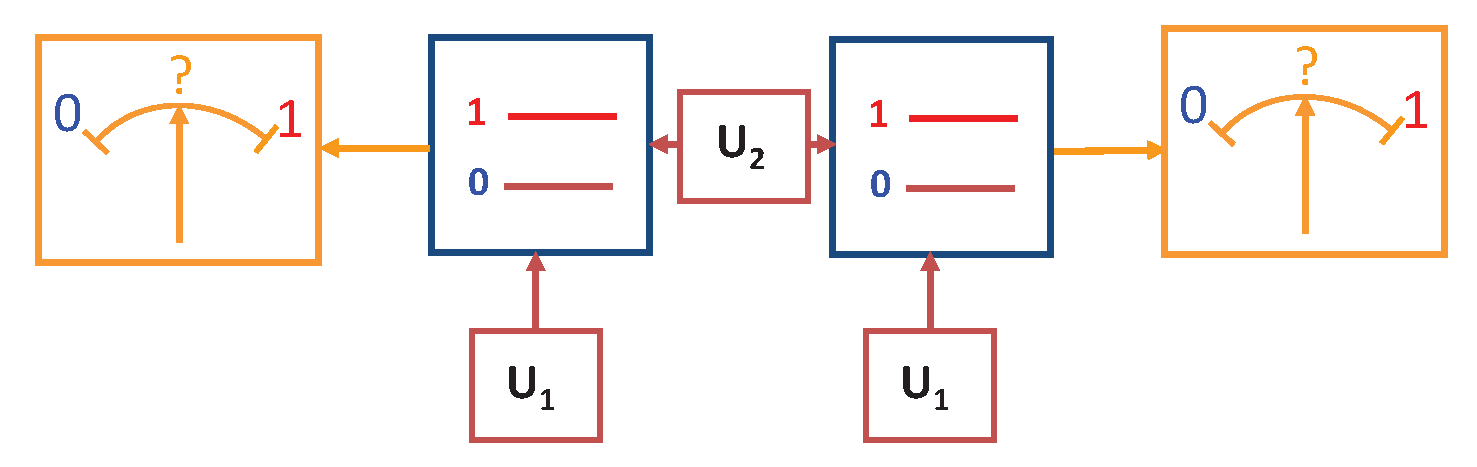
\includegraphics[width=0.8\textwidth]{./material/papers/grover/submission1/Fig1}
	\caption[Blueprint of a 2-qubit quantum processor]{The blueprint of a 2 qubit quantum processor. Shown a two qubits which can be manipulated individually ($U_1$) and which possess a universal two-qubit gate $U_2$. Each of the qubits can be read out individually.}
	\label{fig:Grover1}
\end{figure}

This thesis presents experiments performed on on superconducting 2-Qubit quantum processor. The main goal of this work was to demonstrate a possible quantum computing architecture using superconducting qubits that follows the canonical blueprint of a 2-qubit quantum processor as formulated by \cite{divincenzo_physical_2000} and as shown in fig. \ref{fig:Grover1}. In this respect, a universal quantum computer is a register of quantum bits -- or qubits -- on which one can perform universal 1- and 2-qubit quantum gates. In addition, one can read out the state of each qubit individually and with high fidelity and reset the qubit register to a well-defined product state.

Implementing this allegedly simple list of requirements in a system of superconducting qubits has been a major research challenge during the last decade. The first demonstration of coherent quantum-mechanical dynamics in a superconducting structure by \cite{nakamura_coherent_1999} sparked a broad research field about superconducting quantum bits. In the years following Nakamura's discovery, several types of superconducting qubits were proposed and realized, using the superconducting phase \citep{martinis_energy-level_1985,martinis_rabi_2002} across a Josephson junction or the magnetic flux \citep{mooij_josephson_1999,chiorescu_coherent_2003} in a superconducting ring as the dominant quantum variable. An important result was the development of the so called {\it Quantronium} qubit \citep{vion_manipulating_2002}, which showed for the first time a coherence time larger than 1 $\mu s$ by using an intermediate regime between charge and phase qubits and operating the device at a sweet spot. This made it possible to perform -- for the first time -- robust, high fidelity single-qubit operations with a superconducting qubit \citep{collin_nmr-like_2004}. In 2004, the development of a new type of qubit, the so called {\it Transmon} \citep{wallraff_strong_2004} again drastically improved the reliability of superconducting qubits by operating a Copper pair box deep in the phase regime and embedding it in a superconducting coplanar waveguide resonator. In this so called ``circuit quantum electrodyanmics'' (CQED) approach \citep{blais_cavity_2004} the resonator protects the qubit from electrical noise and at the same time allows a robust readout scheme through its dispersive interaction with the qubit. Within this approach, quantum gates and algorithms with up to four qubits have been realized, demonstrating multi-qubit entanglement \citep{dicarlo_preparation_2010}, simple quantum algorithms \citep{dicarlo_demonstration_2009} and even benchmarks of teleportation protocols \citep{baur_benchmarking_2011}.

In parallel to this, the development of quantum-limited amplifiers based on nonlinear superconducting resonators by \question{Should I mention Michel here?}I. Siddiqi \citep{siddiqi_rf-driven_2004} complemented the CQED architecture by providing a fast and high-fidelity readout scheme for Transmon qubits \citep{siddiqi_dispersive_2006,mallet_single-shot_2009} and for the amplification of quantum signals in general\todo{Add more citations here}. This opened for example the road to the direct observation of quantum jumps in superconducting qubits \citep{vijay_observation_2011} and to implementing simple forms of quantum feedback\todo{Add reference to quantum feedback paper as soon as it appears}.

Another important recent breakthrough was the development of a qubit architecture using three-dimensional superconducting cavitities instead of one-dimensional coplanar waveguide resonators by Paik et. al. \citep{paik_observation_2011}. By combining well-controlled, large Transmon qubits fabricated on a Sapphire substrate with a very high-Q 3D resonator it was possible to obtain an increase of qubit lifetime of one order of magnitude, with values ranging as high as $80 \; \mu \mathrm{s}$\todo{verify this!}. This enormous leap in coherence time will probably make possible the realization of high-fidelity quantum gates and qubit readout schemes as well as elemental quantum feedback and error correction schemes \todo{update this section as soon as new relevant material appears}.

This thesis tries to fit in this global picture by combining the multi-qubit CQED approach to quantum computing with a high-fidelity, single-shot qubit readout mechanism using Josephson parametrics amplifiers. By doing this we want to complement the CQED architecture for superconducting quantum bits with the missing elements from the list of requirements of \cite{divincenzo_physical_2000} and to make possible the construction of a scalable, superconducting qubit quantum processor. 

The first part of this thesis discusses therefore the realization of a superconducting quantum processor that complements the CQED architecture with a per-qubit single-shot readout. We demonstrate elemental 1- and 2-qubit quantum operations on this processor and use it to implement a simple quantum algorithm that can demonstrate quantum speed-up. Afterwards, we discuss the realization of a 4-qubit quantum processor within a more scalable architecture that fulfills -- to varying degree -- all of the diVincenzo criteria and can possibly be extended to a large number of qubits.

\subsection{Realizing a Two-Qubit Quantum Processor}

\begin{figure}[ht!]
	\centering
		\includegraphics[width=0.75\textwidth]{./material/papers/grover/figures/2_qubit_processor_schematic}
	\caption[Circuit schematics of the realized 2-qubit processor]{Circuit schematics of the two-qubit processor realized in this work, showing the two qubits in green, the qubit readouts in blue and the fast flux lines in red. Each qubit is embedded in its own nonlinear readout resonator and can be driven and read out through an individual microwave line. The simultaneous single-shot readout of the two qubits produces measurement outcomes in the basis $x \in \{00,01,10,11\}$.}
	\label{fig:two_qubit_processor_schematic}
\end{figure}

The quantum processor implemented in this work is shown in fig. \ref{fig:two_qubit_processor_schematic}. It consists of two superconducting quantum bits of the Transmon-type, each equipped with its own drive and readout circuit. The qubit readout is realized by using a nonlinear coplanar-waveguide resonator that serves as a Josephson bifurcation amplifier (JBA) and allows for high-fidelity, single-shot readout of the qubit state. Each qubit can be manipulated by driving it with microwave pulses through its readout resonator, allowing us to realize high-fidelity single-qubit operations. In addition, the qubit frequencies can be tuned individually by fast flux lines, which allows for fast frequency control over the range of several GHz for each qubit. The coupling between the two qubits is realized through a fixed capacitor that directly connects the top electrodes of the two qubits and produces a fixed $\sigma_{xx}$-type coupling. This allows us to realize 2-qubit gates and to generate highly entangled 2-qubit states. We can use the processor to test Bell's inequality, implement an universal 2-qubit gate and perform simple quantum algorithms and demonstrate quantum speed-up, as will be shown in the following sections.

\subsection{Demonstrating Simultaneous Single-Shot Readout}

\begin{figure}[ht!]
	\centering
		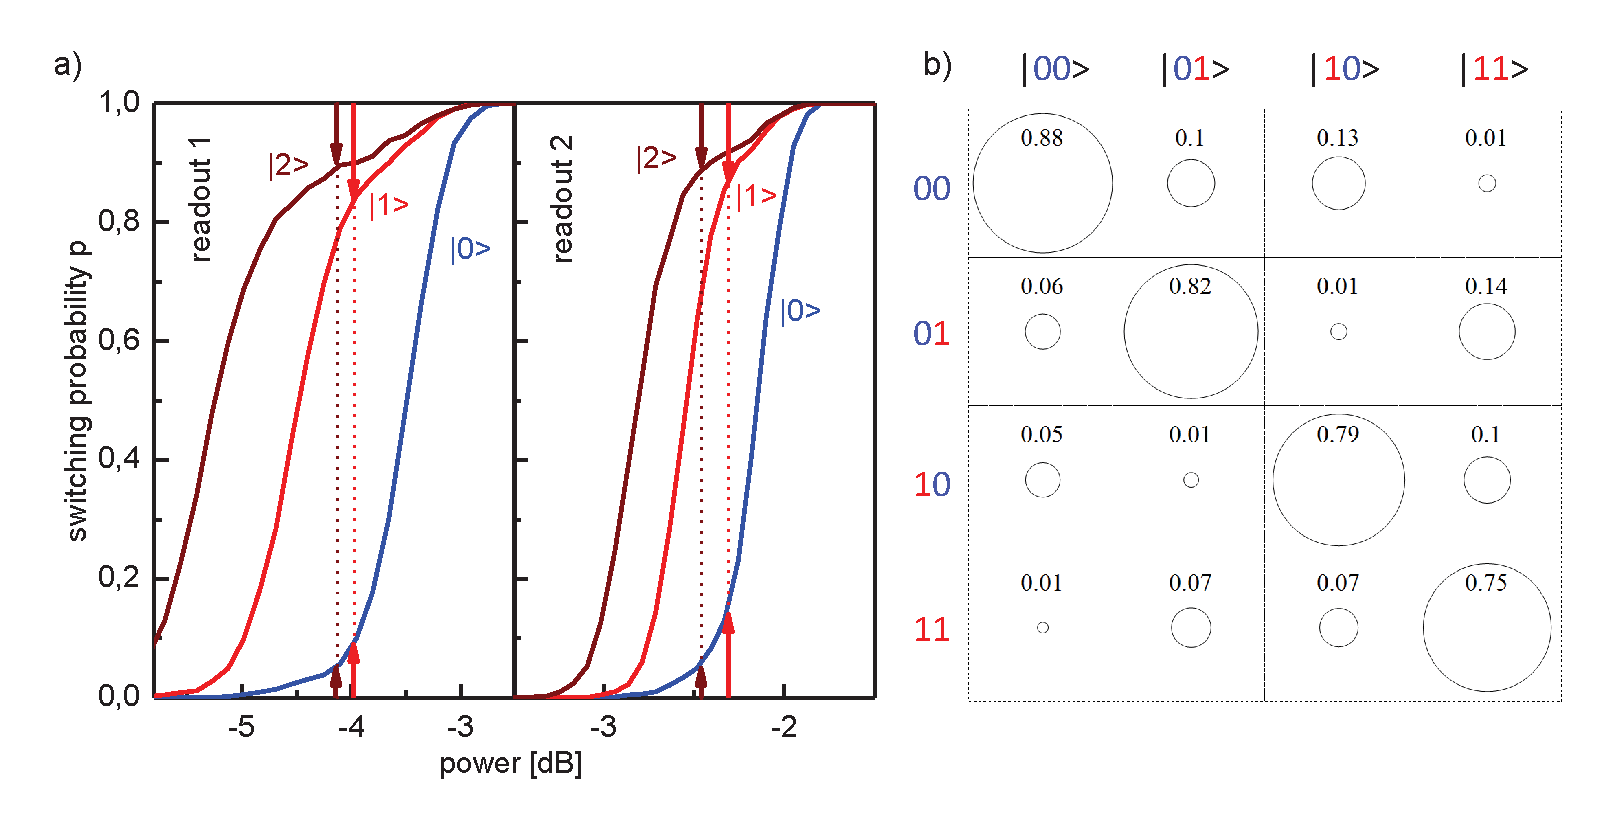
\includegraphics[width=1.\textwidth]{./material/papers/grover/figures/simultaneous_readout_characteristics}
	\caption[Switching probabilities of the two qubit readouts as a function of the readout excitation power]{a) Switching probabilities of the two qubit readouts as a function of the readout excitation power. The measurement is performed after preparing the qubits in the states $\ket{0}$, $\ket{1}$ and $\ket{2}$. The readout fidelity is given as the difference in probability between the curves corresponding to the states $\ket{0}$ and $\ket{1}$ or $\ket{2}$, respectively. The highest readout fidelites of 88 and 89 \% are achieved when the qubit is in state $\ket{2}$. b) Readout matrix of the 2-qubit system. The matrix contains the probabilities of obtaining a given measurement result after having prepared the system in a given state. \figcomment{Replace this figure since it is not very intuitive. It would be better to show something which allows the reader to directly quantify the visibility and readout crosstalk present in the system.}}
	\label{fig:QubitReadoutCharacteristics}
\end{figure}

The read out of the qubit state is done by using a so-called Josephson bifurcation amplifier \citep{siddiqi_dispersive_2006,mallet_single-shot_2009}. This readout works by capacitively coupling the qubit to a coplanar waveguide resonator which is rendered nonlinear by adding a Josephson junction at the center of the resonator. This nonlinear resonator can exhibit bistable behaviour for certain drive parameters, which we can use to map the state of the qubit to one of the bistable states of the resonator, thus obtaining a high-fidelity, single-shot readout of the qubit. In contrast to other CQED architectures, each of the two qubits of our processor possesses its own JBA readout, which follows the diVincenzo criteria by allowing a simultaneous measurement of the state of the whole qubit register. The fidelity attained with a JBA readout can be as high as 93 \% \citep{mallet_single-shot_2009}, but due to design contraints was usually around 83-85 \% for the quantum processor realized here.

\subsection{Generating and Characterizating Entanglement}

\begin{figure}
	\centering
		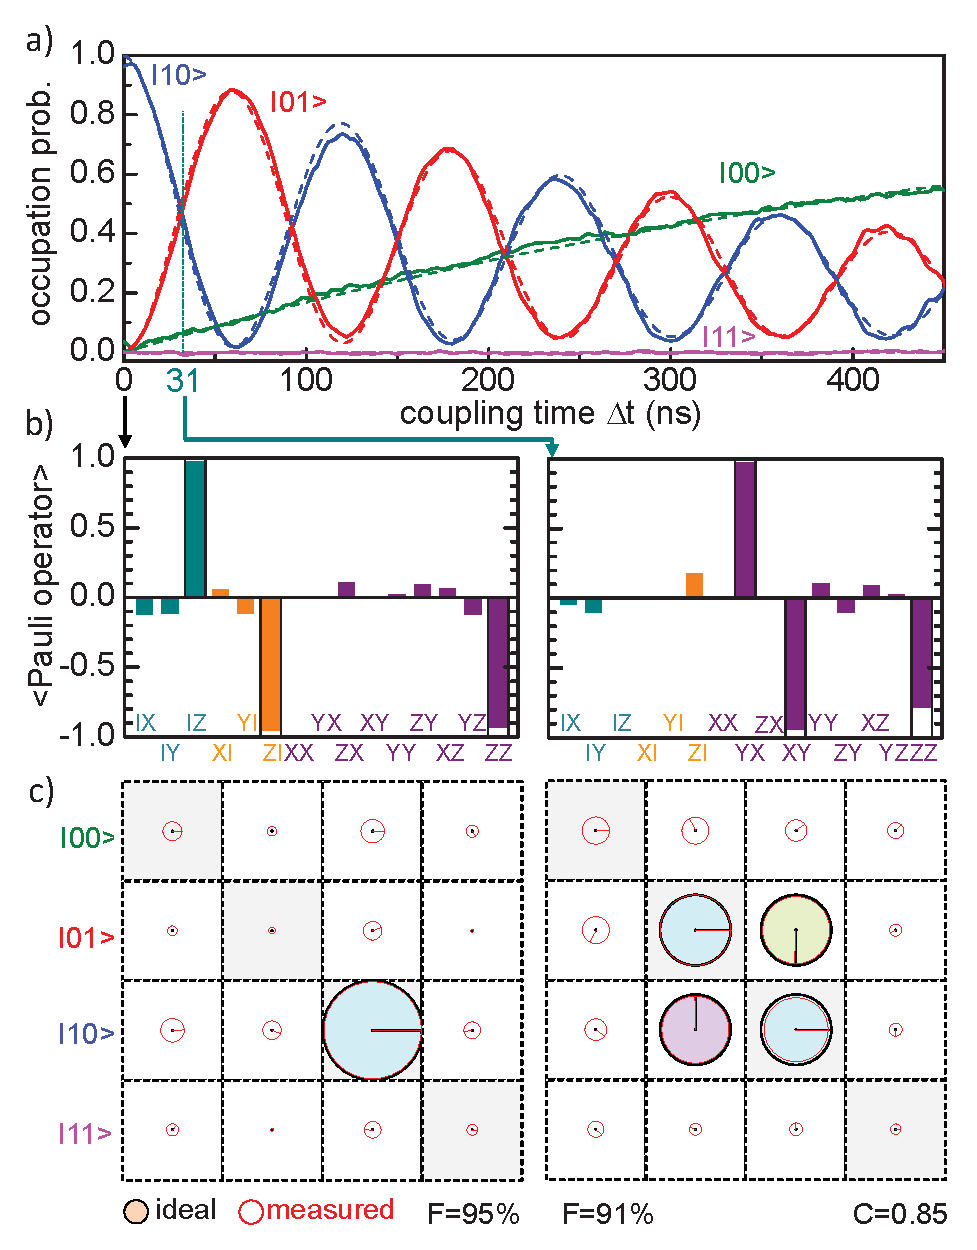
\includegraphics[width=0.7\textwidth]{./material/papers/iswap/submission1/Dewes_Figure2}
	\caption[Generating entangled 2-qubit states by swapping interaction]{An experiment showing the creation of entanglement between the two qubits and the realization of the universal $\sqrt{i\mathrm{SWAP}}$ quantum gate. The qubits start out seperated in frequency and are initialized to the state $\ket{10}$. Afterwards, the qubit frequencies are non-adiabatically tuned into resonance and held there for a well-defined time $\Delta t$. When measuring the $\sigma_z^1 \otimes \sigma_z^2$ operator of the system, an energy exchange between the states $\ket{01}$ and $\ket{10}$ can be observed. The reconstruction of the full quantum state of the system after an interaction time of $\Delta t = 31 \; \mathrm{ns} $ by quantum state tomography shows entanglement between the qubits. By adding compensating $\sigma_z^{1,2}$ pulses after the application of the entanglement gate one can implement the $\sqrt{i\mathrm{SWAP}}$ gate.}
	\label{fig:iSwap2}
\end{figure}

The fixed coupling between the two qubits of our processor provides a $\sigma_{xx}$-type coupling of the qubits. This coupling is effective only when the qubit frequencies are near-resonance and can thus be switched on and off by changing the qubit frequencies. In the processor presented in this work, the effective coupling constant $g$ of the qubits was of the order of $2g = 8.2 \; \mathrm{MHz}$\todo{Check if this is really $2g$!}. When this coupling is switched on non-adiabatically -- e.g. by abruptly tuning the two qubits into resonance --, the evolution operator of the coupled 2-qubit system takes the form

\begin{equation}
	U(t)  =  \left( \begin{array}{cccc} 1 & 0 & 0 & 0 \\ 0 & \cos{2 \pi t g} & i\sin{2 \pi t g} & 0 \\ 0 & i\sin{2 \pi t g} & \cos{2 \pi t g} & 0 \\ 0 & 0 & 0 & 1 \end{array} \right) \label{eq:swap_evolution_operator}
\end{equation}

This evolution allows for the generation of entangled 2-qubit states.\comment{First discuss the dynamics of the SWAP} For this, we start in the state $\ket{00}$ and use a single-qubit pulse to generate the state $\ket{10}$. When switching on the interaction between the qubits as given in eq. (\ref{eq:swap_evolution_operator}) for a given amount of time we can observe oscillations in the state of the 2-qubit system as a function of the interaction time, as shown in fig. \ref{fig:iSwap2}a. When stopping the interaction after the right amount of time we can create highly entangled 2-qubit states, which we can then characterize by using quantum state tomography. The experimental reconstruction of the density matrix of a Bell-type state of the form $\ket{\psi} = 1/\sqrt{2}(\ket{01}+i\ket{10})$ created by this method is shown in fig. \ref{fig:iSwap2}b. The fidelity of the experimentially measured state with the ideal Bell-state is 91 \%, the concurrence of the state is 85 \%, indicating a high amount of entanglement. Besides performing quantum state tomography, we can also characterize the entanglement of this state by performing a Clauser-Horne-Shimony-Holt experiment\citep{clauser_proposed_1969}, where we measure the expectation value of the quantity

\begin{equation}
\mathrm{CHSH} = \mathrm{QS}+\mathrm{RS}+\mathrm{RT}-\mathrm{QT}
\end{equation}
, where the operators $\mathrm{Q,R,S,T}$ are given as

\begin{eqnarray}
	\begin{array}{cccccccc}
		\mathrm{Q} & = & \sigma_z^1 &&& \mathrm{S} & = & \sigma_z^2\cdot \cos{\phi}+\sigma_x^2 \cdot \sin{\phi} \\
		\mathrm{R} & = & \sigma_x^1 &&& \mathrm{T} & = & -\sigma_z^2\cdot \sin{\phi}+\sigma_x^2 \cdot \cos{\phi}
	\end{array}
\end{eqnarray} 

\begin{figure}[ht!]
	\centering
		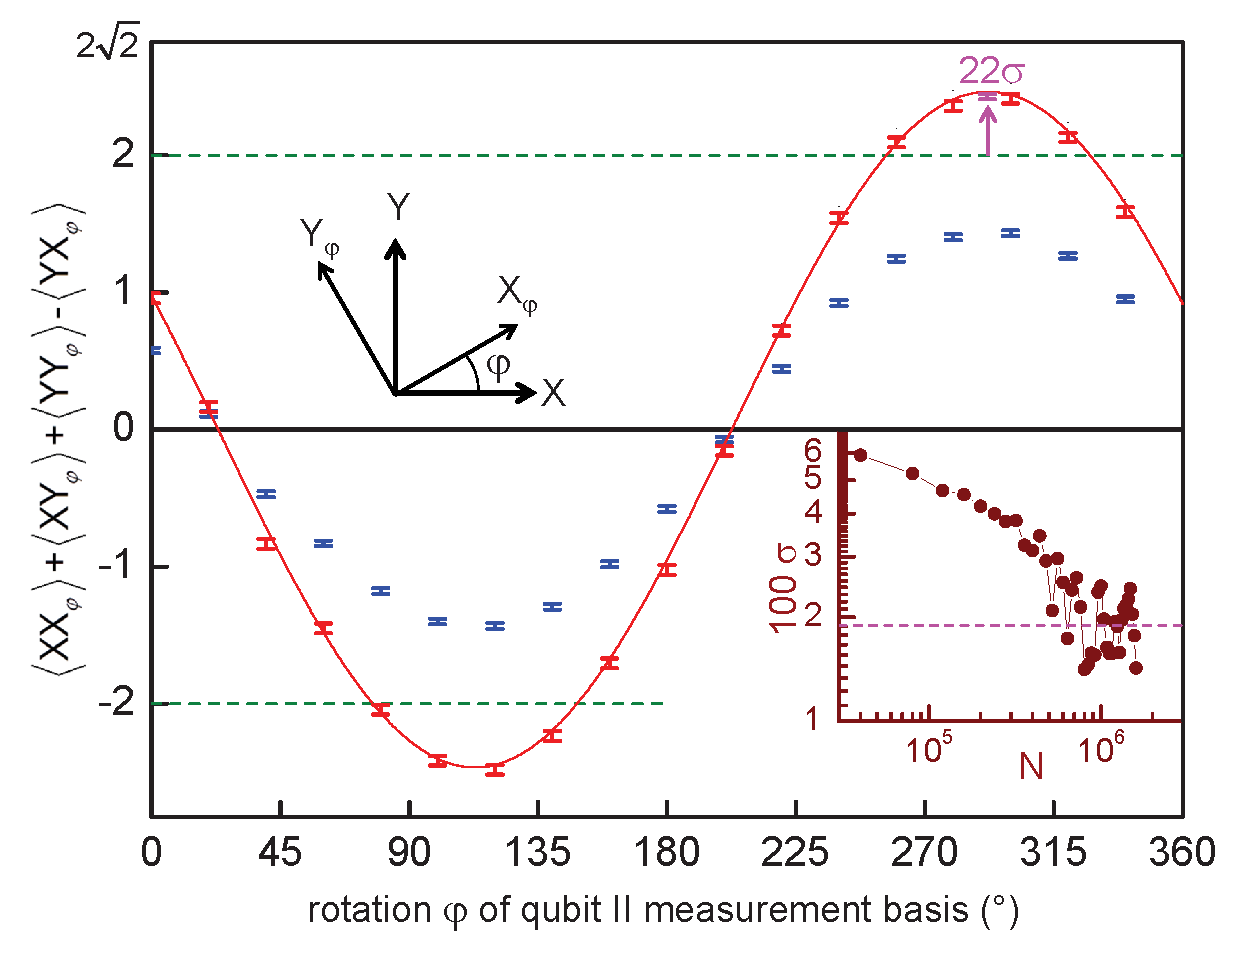
\includegraphics[width=0.7\textwidth]{./material/papers/iswap/submission1/Dewes_Figure3}
	\caption[Measurement of the CHSH operator of an entanged 2-qubit state]{Measurement of the CHSH equation for an entangled 2-qubit state. The renormalized CHSH expectation value exceeds the classical boundary of $2$. Due to limited readout visibility, the raw measurement data (blue data points) lies below this critical threshold. The inset shows the standard deviation $\sigma$ at the highest point of the curve as a function of the sample size. For the highest sample count, the classical boundary is exceeded by $22$ standard deviations.\figcomment{p. 140 in cavities 6 labbook}}
	\label{fig:chsh_measurement}
\end{figure}

The expectation value $\bracket{CHSH}(\phi)$ will reach a maximum value of $\sqrt{2}\cdot 2$ for a superposition state $1/\sqrt{2}(\ket{01}+e^{i\phi}\ket{10})$ and provides a test of the quantum-mechanical character of the generated state. The result of a CHSH-type of measurement performed with our quantum processor is shown in fig. \ref{fig:chsh_measurement}. When correcting for readout errors, we observe a violation of the classical boundary $2$ by $22$ standard deviations. However, due to limited readout visibility we do not violate Bell's inequality for the uncorrected, raw data. Our measurement can therefore not serve as a definite proof of quantum mechanical behaviour in our system but nevertheless provides a strong indication of the presence of entanglement in the state that we characterized.

\subsection{Realizing a Universal Two-Qubit Quantum Gate}

\begin{SCfigure}[][ht!]
		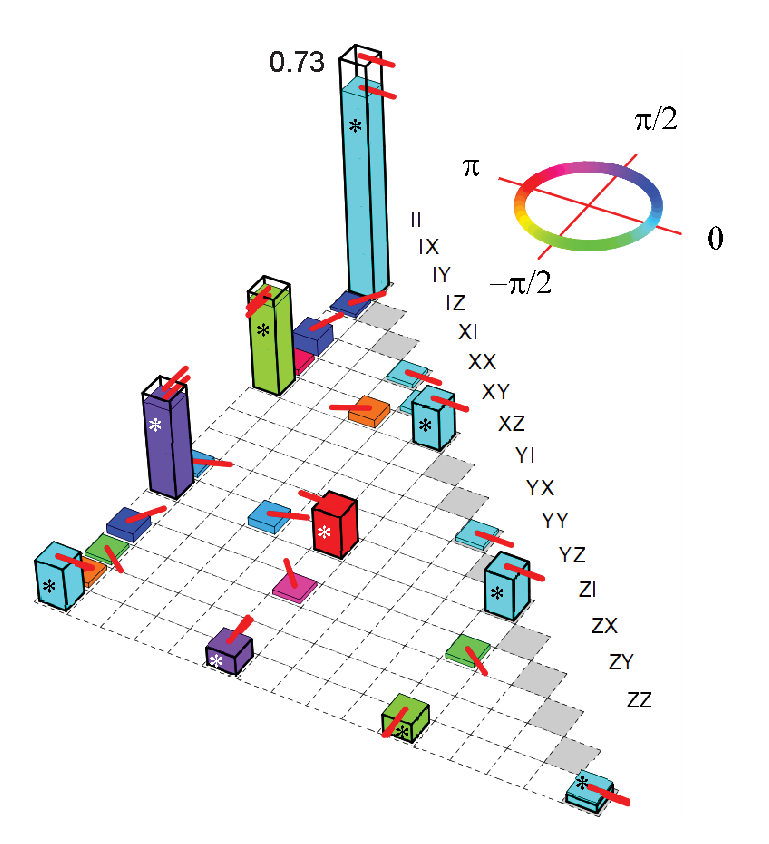
\includegraphics[width=0.65\textwidth]{./material/papers/iswap/figures/chi_matrix}
	\caption[Experimental $\chi$-matrix of the implemented $\sqrt{i\textrm{SWAP}}$ gate]{The experimentally measured $\chi$-matrix of the implemented $\sqrt{i\mathrm{SWAP}}$ gate. The row labels correspond to the indices of the $E_i$ operators, the height of each bar gives the absolute value of the corresponding matrix element, the complex phase is indicated by color and the red arrow. The ideal $\chi$-matrix of the gate is given by the outlined bars.}
	\label{fig:GateChiMatrixAndErrorProcess}
\end{SCfigure}

When letting the qubits evolve according to eq. (\ref{eq:swap_evolution_operator}) for exactly $t = 1/8g$ one obtains the so called $\sqrt{i\mathrm{SWAP}}$ gate, which has the representation

\begin{equation}
	\sqrt{i\mathrm{SWAP}}  =  \left( \begin{array}{cccc} 1 & 0 & 0 & 0 \\ 0 & 1/\sqrt{2} & i/\sqrt{2} & 0 \\ 0 & i/\sqrt{2} & 1/\sqrt{2} & 0 \\ 0 & 0 & 0 & 1 \end{array} \right) \label{eq:sqrt_iswap_gate}
\end{equation}

The pulse sequence used to realize this quantum gate is shown in fig. \ref{fig:iSwap2}.  The attained fidelity of this gate was 90 \% for the realized quantum processor, which is goog enough to allow a simple demonstration of a benchmark quantum algorithm with the system.

\subsection{Running a Quantum-Search Algorithm}

\begin{figure}[ht!]
	\centering
		\includegraphics[width=0.8\textwidth]{./material/papers/grover/figures/grover_algorithm_schematic}
	\caption[Schematic of our implementation of Grover's search algorithm]{Our implementation of Grover's search algorithm for a 2-qubit quantum processor. The algorithm consists in preparing a probe state, applying the quantum oracle to this state and analyzing the resulting output state to find out which oracle has been applied to it. A single run of the algorithm -- and thus a single evaluation of the oracle function -- suffices to obtain the full information on the oracle operator with 100 \% theoretical success probability.}
	\label{fig:GroverAlgorithmSchematic}
\end{figure}

The demonstration of quantum speed-up is an important benchmark for any prospective quantum processor. In this work, we implemented a compiled version of Grover's search algorithm \citep{Grover_Quantum_1997}. Our version of the algorithm works in the basis of two qubits $x_i \in \{\ket{00},\ket{01},\ket{10},\ket{11}\}$ and in theory can distinguish between four different ``oracle functions'' $f(x)$ which mark a given state $x_j$ and leave the other states unchanged. Since the algorithm requires only one evaluation of the function $f(x)$ to determine which state has been marked it is 50 \% faster than any conceivable classical algorithm\comment{discuss again if this should be 25 \% or 50 \%}. 

\subsection{Demonstrating Quantum Speed-Up}

In the last section we discussed the implementation of Grover's search algorithm using our quantum processor and how we can characterize the operation of the algorithm using quantum state tomography. However, the main interest of running a quantum algorithm is to obtain an advantage in the run-time as compared to a classical algorithm, the so-called ``quantum-speedup''. To characterize this quantum speed-up as obtained with our processor, we simply run Grover's algorithm for all four possible oracle functions and directly look at the outcome of the final readout step, \textit{without} correcting for readout errors or performing additional tomography steps. By averaging the results of individual runs of our processor we can thus obtain the so-called single-run fidelity, which ranges between 52 and 67 \%, depending on the state marked by the given quantum oracle. This results therefore clearly demonstrates quantum speed-up in this system, although the achieved success probability is considerably lower than the theoretically possible value of 100 \% .

\begin{figure}[ht!]
		\centering
		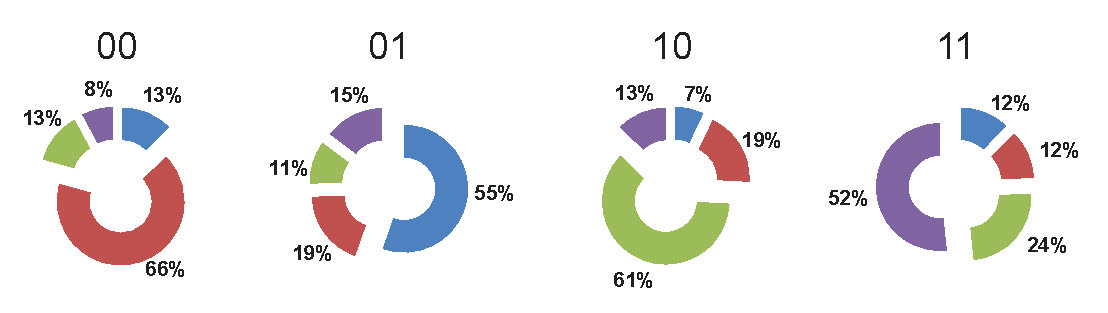
\includegraphics[width=1.0\textwidth]{./material/papers/grover/figures/grover_algorithm_single_shot_probabilities}
	\caption[Single run results of Grover's search algorithm implemented on our quantum processor]{Single-run results when running Grover's search algorithm on our quantum processor. Shown are the probabilities of obtaining the results $00,01,10,11$ depending on the oracle function given to the algorithm (shown on top). In all four cases, the success probability of the algorithm is $> 50 \%$, thus outperforming any classical algorithm in the number of calls to the oracle function.}
	\label{fig:GroverSingleShotProbabilities}
\end{figure}

\subsection{Designing a Scalable Quantum Computing Architecture}

After having demonstrated the different building blocks of a superconducting, Transmon-based quantum processor it remains to be shown that larger-scale quantum-computing beyond two qubits is possible with this system. This work therefore pursued the realization of a more scalable qubit architecture using systems of up to six qubits coupled through a so-called ``quantum bus'' \citep{majer_coupling_2007}. The details of this novel architecture are discussed in the following sections.

The approach for scalable quantum computing with superconducting qubits pursued in this work consists of a system of many individual Transmon qubits equipped with individual JBA-based readouts, a multiplexed drive and readout circuit and a fixed qubit-qubit coupling mediated through a high-Q CPW resonator. As before, each qubit possesses a fluxline for fast frequency control. The readout and drive signals are send to all the qubits in parallel through a multiplexed 50 $\Omega$ transmission line. In this approach, the frequencies of the JBA readouts have to be chosen such that driving individual readouts at a given frequency does not induce crosstalk or spurious coupling to other readout resonators. Also, the transition frequencies of all qubits have to be chosen such that it becomes possible to individually address each of them without inducing transitions in the other qubit states.
